\documentclass{beamer} 
\usetheme{msu}
\usepackage{xcolor} 
\usepackage{tikz}
\usetikzlibrary{calc}
\usepackage{xifthen}
\usepackage{subfig}
\usepackage{pgfplots}
\usepackage{animate}
\usepackage{algorithm}
\usepackage{algpseudocode}
\pgfplotsset{compat=newest}

\newcommand*{\overlaynumber}{\number\beamer@slideinframe}

\usepackage{pgfpages}
%\pgfpagesuselayout{4 on 1}[a4paper,border shrink=5mm]

% Beamer setup
\AtBeginSection[]
{
  \begin{frame}
    \frametitle{Table of Contents}
    \tableofcontents[currentsection]
  \end{frame}
}
%\setbeamertemplate{headline}{}

\setbeamertemplate{headline}
{%
  \leavevmode%
  \begin{beamercolorbox}[wd=.5\paperwidth,ht=2.5ex,dp=1.125ex]{section in head/foot}%
    \hbox to .5\paperwidth{\hfil\insertsectionhead\hfil}
  \end{beamercolorbox}%
  \begin{beamercolorbox}[wd=.5\paperwidth,ht=2.5ex,dp=1.125ex]{subsection in head/foot}%
    \hbox to .5\paperwidth{\hfil\insertsubsectionhead\hfil}
  \end{beamercolorbox}%
}

% Algorithmic parallel commands
\algblock{ParFor}{EndParFor}
\algnewcommand\algorithmicparfor{\textbf{parfor}}
\algnewcommand\algorithmicpardo{\textbf{do}}
\algnewcommand\algorithmicendparfor{\textbf{end\ parfor}}
\algrenewtext{ParFor}[1]{\algorithmicparfor\ #1\ \algorithmicpardo}
\algrenewtext{EndParFor}{\algorithmicendparfor}

% Algorithmic parallel commands
\algblock{RedParFor}{EndRedParFor}
\algnewcommand\algorithmicredparfor{{\color{red}\textbf{parfor}}}
\algnewcommand\algorithmicredpardo{{\color{red}\textbf{do}}}
\algnewcommand\algorithmicendredparfor{{\color{red}\textbf{end\ parfor}}}
\algrenewtext{RedParFor}[1]{\algorithmicredparfor\ #1\ \algorithmicredpardo}
\algrenewtext{EndRedParFor}{\algorithmicendredparfor}
%\usetikzlibrary{decorations.pathreplacing}
%\usetikzlibrary{plotmarks}

\logo{
\includegraphics[height=2cm]{msu_seal_washout}} 

\title[Pipeline Schwarz Waveform Relaxation\hspace{1em}\insertframenumber/
\inserttotalframenumber]{~ Pipeline Schwarz Waveform Relaxation ~}

\author[Scott High \quad highscot@msu.edu \qquad SIAM Parallel, 2014]{Benjamin Ong \inst{1} \and Scott
  High \inst{1} \and \\Felix Kwok \inst{2}}
\institute[shortinst]{\inst{1} Michigan State University, East
  Lansing, MI \and \inst{2} Universit\'{e} de Gen\`{e}ve, Switzerland }

\date{\today}

\makeatletter
\newcommand{\cemph}[1]{{\color[rgb]{1,0,0} \emph{#1}}}

\define@key{beamerframe}{t}[true]{% top
  \beamer@frametopskip=.2cm plus .5\paperheight\relax%
  \beamer@framebottomskip=0pt plus 1fill\relax%
  \beamer@frametopskipautobreak=\beamer@frametopskip\relax%
  \beamer@framebottomskipautobreak=\beamer@framebottomskip\relax%
  \def\beamer@initfirstlineunskip{}%
}

\begin{document}

\begin{frame}{Waveform levels figure}
  
  \begin{figure}
    \centering
    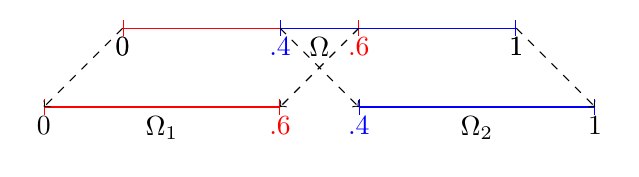
\begin{tikzpicture}

      \only<1>
      {
        \draw[|-|] (3,2) -- (8,2)
        node[pos=0, below]{$0$}
        node[pos=.5,below]{$\Omega$}
        node[pos=1, below]{$1$};
      }

      \onslide<2->
      {
        \draw[|-|,color=red] (3,2) -- ++(3,0)
        node[pos=0, below, color=black]{$0$}
        node[pos=1, below]{$.6$};
        
        \draw[|-|,color=blue] (5,2) -- ++(3,0)
        node[pos=0, below]{$.4$}
        node[pos=1, below, color=black]{$1$};

        \draw[|-|,color=red] (2,1) -- (5,1)
        node[pos=0, below, color=black]{$0$}
        node[pos=.5,below, color=black]{$\Omega_1$}
        node[pos=1, below]{$.6$};

        \draw[|-|,color=blue] (6,1) -- (9,1)
        node[pos=0, below]{$.4$}      
        node[pos=.5,below, color=black]{$\Omega_2$}
        node[pos=1, below, color=black]{$1$};      

        \draw[->,dashed] (5,2) -- (6,1);
        \draw[->,dashed] (8,2) -- (9,1);
        \draw[->,dashed] (6,2) -- (5,1);
        \draw[->,dashed] (3,2) -- (2,1);
      }
    \end{tikzpicture}
  \end{figure}

  
\end{frame}


\end{document}
